\section{Semantic Concentrator}
\label{sec:sec}


The \textbf{Semantic Concentrator (SEC)} enhances inference efficiency by selectively retaining semantically important visual tokens based on language context. 
It operates in the attention layers and consists of three tightly coordinated yet modular components, as shown in \Fig{fig:semantic}:
The \textbf{importance analyzer} that estimates the importance of visual tokens based on cross-modal attention.
A lightweight \textbf{top-$k$ sorter} that identifies the most important image tokens on the fly.
An \textbf{offset encoder} that enables lossless index tracking for streaming token recovery.
 

\subsection{Streaming Importance Analyzer}

{The SEC integrates directly into the attention {$Softmax(QK^T)$} computation pipeline}. As shown in \Fig{fig:semantic}(1), for each attention head, it compute a {$Softmax(QK^T)$} matrix containing four blocks: image-to-image ($M \times M$), image-to-text, text-to-image ($T \times M$), and text-to-text. 
We extract the \textit{Text-to-Image} block ($T \times M$) as the cross-modal importance matrix $I$, where $M$ and $T$ represent the number of image and text tokens, respectively.
To estimate the importance of each image token $j$ over $n$ heads, we compute the maximum attention score it receives from any text token and all heads:
$
s_j = \max_{\substack{1 \leq k \leq n \\ 1 \leq i \leq T}} I^{(k)}_{i,j}
$.
This results in an importance vector of shape $1 \times M$ across all heads. {An on-chip buffer of 25 KB is used to store the importance vector.}

As depicted in \Fig{fig:semantic}(2), the importance analyzer uses {$a$ parallel max units to process the output of the attention \texttt{SoftMax} (provided by the special function unit).} To match throughput, {$a$ max units processes $a$ attention scores concurrently}. This streaming design supports two dataflows:
\textbf{Parallel (spatial) stream}: Attention columns are streamed directly into max units.
\textbf{Orthogonal (temporal) stream}: Attention rows are buffered locally, enabling column-wise reduction.

This fully streaming design ensures minimal area and latency overhead. Since no global operations are needed, the analyzer is decoupled from the main compute path and incurs negligible runtime cost.

\begin{figure}[t]
    \centering
    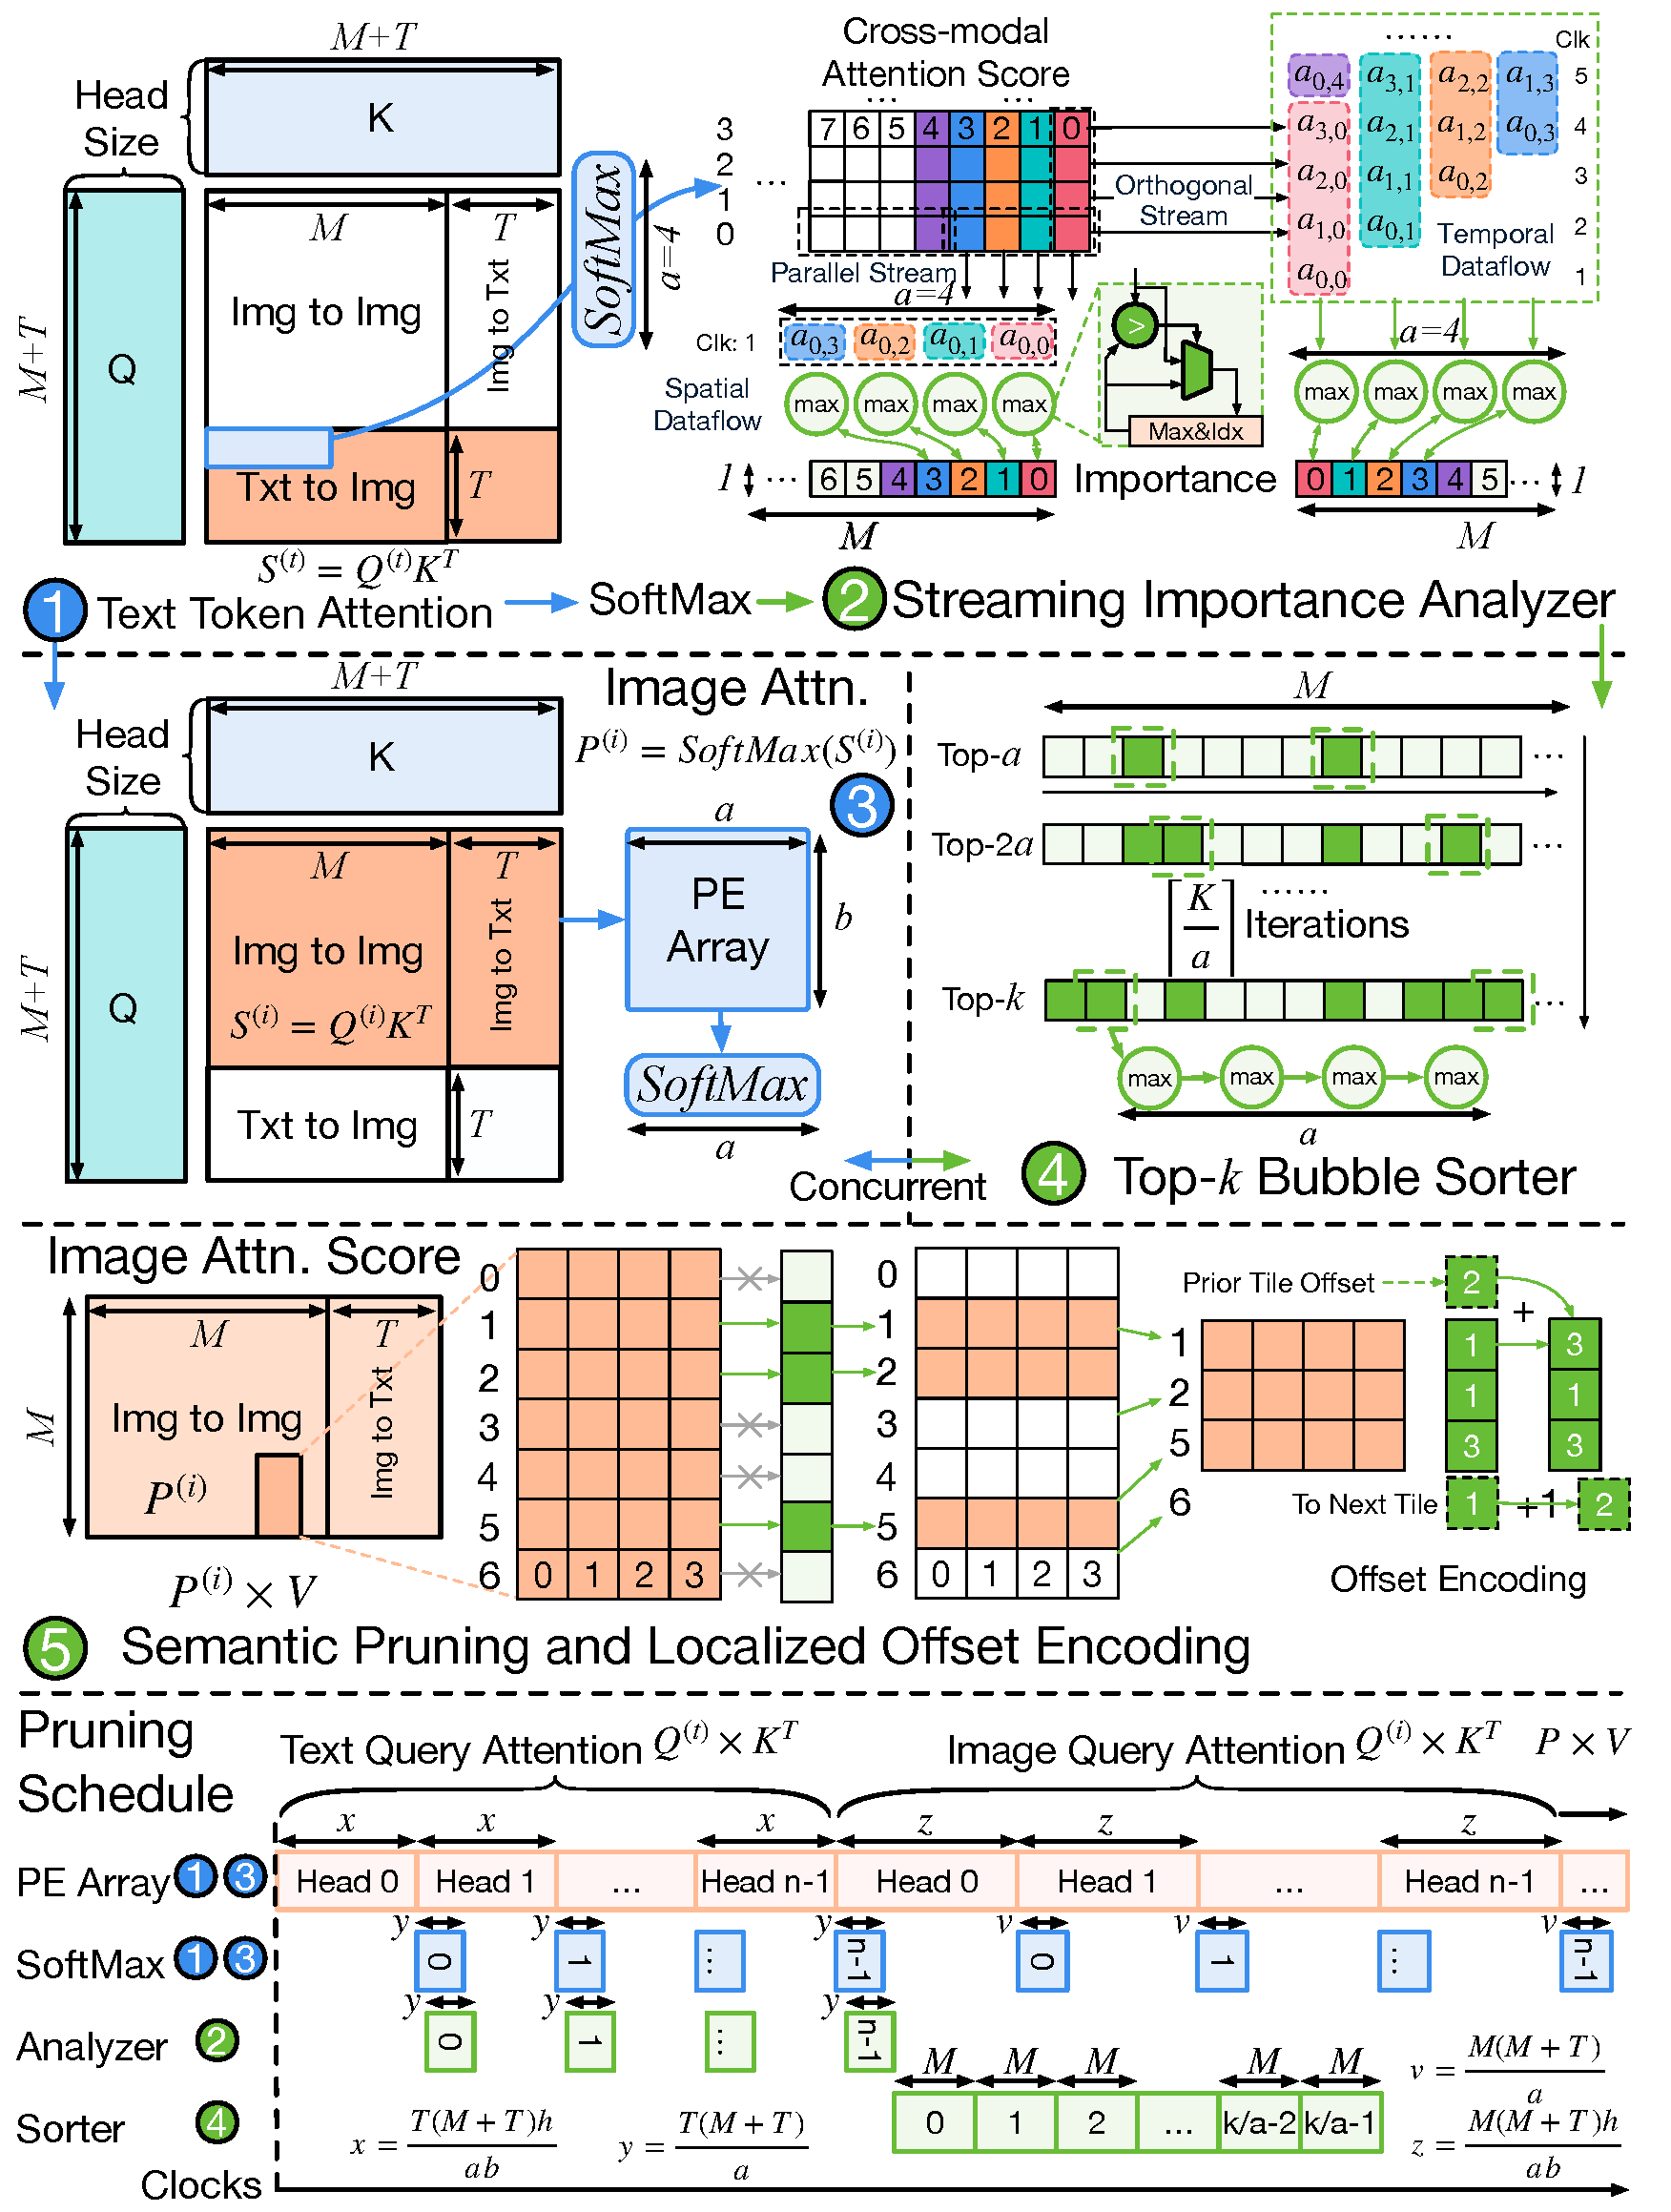
\includegraphics[width=\linewidth]{figure/semantic.pdf}
    % \vspace{-6mm}
    \caption{{Overview of the Semantic Concentrator (SEC), including the streaming importance analyzer, top-$k$ sorter, and offset encoder.}}
    \label{fig:semantic}    
    % \vspace{-5mm}
\end{figure}

\subsection{Top-$k$ Bubble Sorter}

Once the $1 \times M$ importance vector is computed, the system must identify the top-$k$ most relevant tokens. To avoid sorting all $M$ tokens globally, SEC adopts a pipelined bubble sorter as shown in \Fig{fig:semantic}(4).
By chaining the $a$ max units used earlier, we construct an $a$-way streaming bubble sorter. This structure incrementally refines the top-$a$ tokens, allowing us to compute top-$k$ selection over the $M$ candidates in $\frac{M \cdot k}{a}$ cycles, substantially more efficient than full sorting.

Crucially, this process is fully overlapped with the computation of image attention {($S^{(image)} = Q^{(image)}K^T$)}, which dominates the overall runtime.
Let the image attention (within {$QK^T$} GEMM) require $\frac{M \cdot (M+T) \cdot h \cdot n}{a \cdot b}$ cycles, where $h$ is the head dimension, $n$ is the number of heads, and $a \times b$ is the PE array size. The ratio of attention to the sorting operation is:
$
\frac{M \cdot (M+T) \cdot h \cdot n}{a \cdot b} \cdot \frac{a}{M \cdot k} = \frac{(M+T) \cdot h \cdot n}{k \cdot b}.
$
In typical configurations, $h \cdot n$ reaches into the thousands (e.g., 3584), while $b$ is much smaller (e.g., 32) and $k < (M + T)$. Therefore, the sorting operation completes well before the {$Q^{(i)}K^T$} finishes, ensuring that the SEC remains off the critical path and introduces no runtime bottleneck. {A scheduling diagram is shown in \Fig{fig:semantic} bottom to better understand the overlapping.}



\begin{figure*}[t]
    \centering
    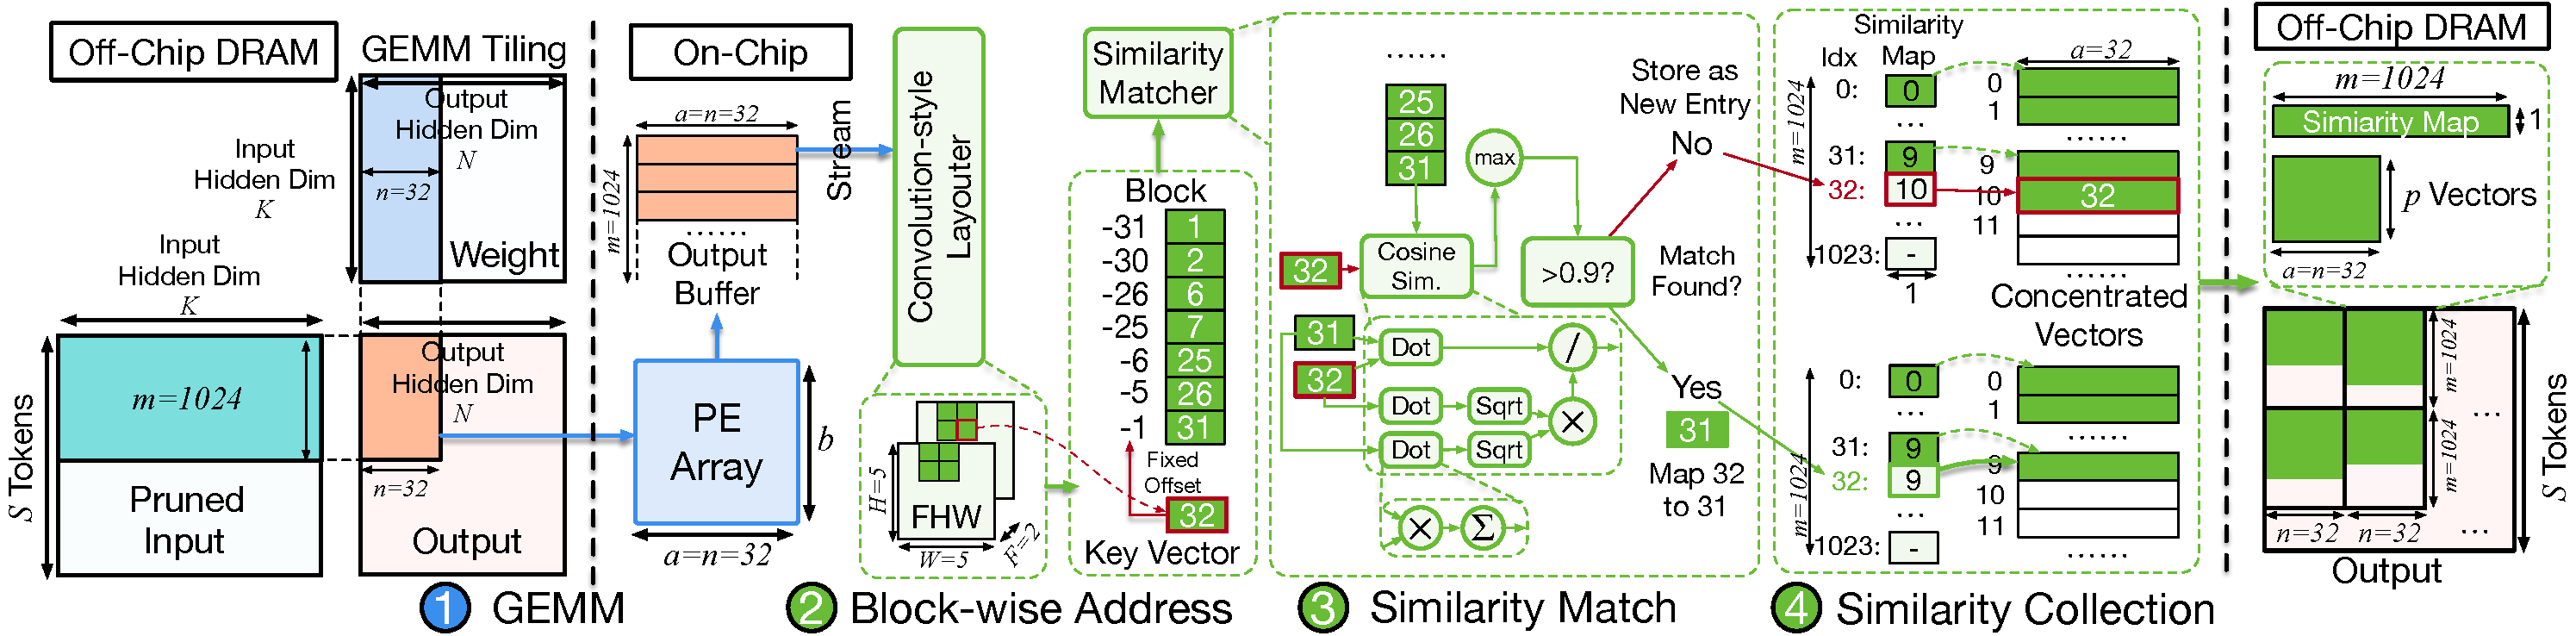
\includegraphics[width=0.99\linewidth]{figure/sic_gather.pdf}
    % \vspace{-3mm}
    \caption{
    Overview of the Similarity Gather module. (1) GEMM tiling. (2) Convolution-style layout reorders outputs into a block-wise structure. (3) Cosine similarity is computed within blocks to detect and eliminate duplicates. (4) Only unique vectors are stored, while a similarity map enables reconstruction.
    }
    \label{fig:sic_gather}
    % \vspace{-5mm}
\end{figure*} 

\subsection{Semantic Pruning and Offset Encoding}
\label{subsec:offset_encoding}
After identifying the top-$k$ most important tokens, we apply \textbf{semantic pruning} for the input of the subsequent attention operation, $P^{(i)}\times V$. 
As shown in \Fig{fig:semantic}(5), only the retained tokens are loaded and processed in $P^{(i)}\times V$, eliminating the need for any memory access or computation on pruned tokens.

In pure pruning mode, no additional metadata is needed. 
However, to support later stages (e.g., similarity concentration), we must record the position of retained tokens for spatial-temporal information. 
For this, the SEC generates \textbf{localized offset encodings}.
The offset encoder, shown in \Fig{fig:semantic}(5), operates in a sliding window over the retained tokens. 
For each token, it records a small integer representing its offset to the previous token. 
This compact encoding is sufficient to restore positional alignment for future operations (e.g., similarity matching).
The encoder's computation is local and streaming, requiring only lightweight registers and no global memory access. 


Overall, the entire Semantic Concentrator, including the analyzer, sorter, and encoder, is fully modular and incurs minimal overhead.
SEC selectively retains the most informative visual tokens using cross-modal attention, top-$k$ selection, and compact position encoding. 
It operates transparently within the attention, requires no additional global memory access, and introduces negligible runtime or area overhead.